\documentclass[class=book, crop=false, oneside]{standalone}
\usepackage[subpreambles=true]{standalone}

\graphicspath{{./assets/diagrams/}}

\begin{document}

\chapter*{Translating ER into RM}
The best way to learn this mechanism is to poceed by examples.\\
Let's start with this one:

\begin{figure}[H]
	\centering
	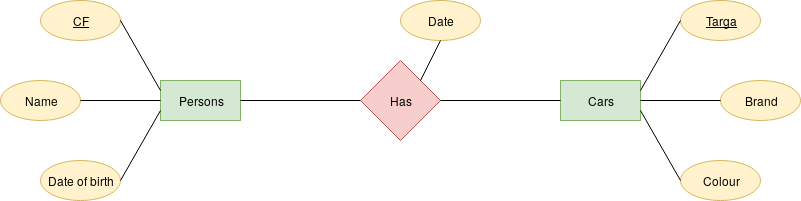
\includegraphics[width=.9\textwidth,keepaspectratio]{diagram1.png}
	\caption{}
	\label{diagram1}
\end{figure}

When we want to translate an ER diagram into an RM model we have to follow certain rules, let's check them out.
\paragraph*{Rule \#1} every entity becomes a table and its attributes are the table's columns.
\paragraph*{Rule \#2} each relation becomes a table and its attributes are part of the table's columns, also the keys of the entities involved in the relation become columns and they are flagged as Foreign Keys(FK).

\end{document}
